% !TeX root = ../FoodSpy.tex
% \section{Descrierea aplicației}

\begin{figure}[!htb]
	\centering
	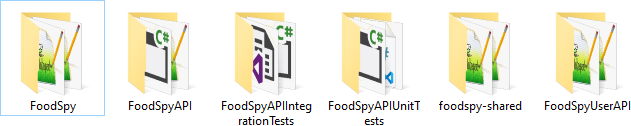
\includegraphics[width=0.8\textwidth]
	{../LaTeX/Images/implementare_arhitectura.PNG}
	\caption{Arhitectura aplicației FoodSpy}
	\label{fig:61}
\end{figure}

Arhitectura aplicației FoodSpy presupune o implementare realizată pe mai multe nivele de infrastructură, nivele ce sunt detaliate în rândurile următoare.
\\ \\
Proiectul ”FoodSpy” reprezintă nivelul clientului sau nivelul de prezentare, adică interfața grafică prin care utilizatorul interacționează cu aplicația.
\\ \\
”FoodSpyUserAPI” este interfața de programare care efectuează comunicarea cu server-ul care se ocupă de administrarea utilizatorilor și a datelor acestora.
\\ \\
Proiectul care se ocupă de persistența datelor reținute în jurnalul fiecărui utilizator este ”FoodSpyAPI”. Acesta este responsabil pentru stocarea informațiilor legate de mâncărurile pe care utilizatorii le pot folosi pentru a-și compune mesele și pentru a înregistra aportul caloric în jurnal.
\\ \\
Nivelul de testare este acoperit de proiectele ”FoodSpyAPIIntegrationTests” și ”FoodSpyAPIUnitTests”.
\\ \\
”foodspy-shared” este proiectul care reprezintă nivelul auxiliar, un nivel care face posibilă partajarea dependințelor aplicației. Acesta conține o colecție de enumerări și interfețe care sunt folosite atât la nivelul clientului cât și la nivelul interfețelor de programare (API-urilor).

\section{Clientul}
Nivelul clientului este împărțit pe mai multe componente Angular.
\\ \\
”Auth” constituie componenta care administrează pagina de autentificare în aplicație. La baza acestei componente este un formular HTML. Pentru un utilizator care urmează să își creeze un cont, formularul are 3 câmpuri: e-mail-ul, parola și aportul zilnic de calorii pe care acesta dorește să-l atingă în fiecare zi. Pentru e-mail se folosește o validare bazată pe o expresie regulată care impune în componența sa existența unui domeniu (”.com”, ”.ro”, etc.). Parola trebuie să aibă un număr minim de caractere, număr definit de o constantă, iar aportul este exprimat ca un număr întreg cuprins într-un anumit interval.
\\ \\
Pentru cazul în care utilizatorul are deja cont și efectuează operația de autentificare în aplicație, formularul nu mai afișează câmpul numărului de calorii.
Se observă astfel faptul că același formular este folosit pentru procesul de înregistrare, dar și pentru procesul de autentificare. Această implementare este posibilă folosind directiva ”*ngIf”.

\begin{figure}[!htb]
	\centering
	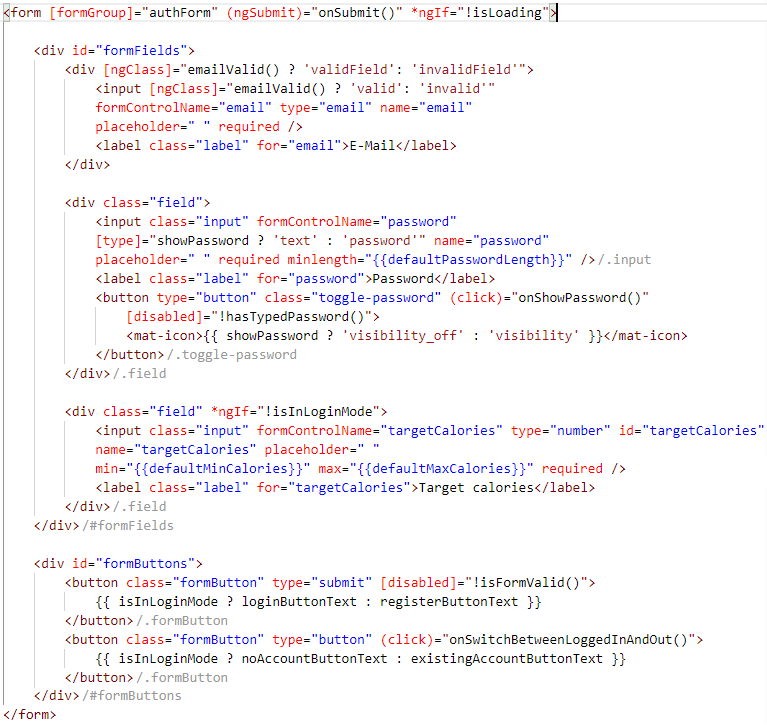
\includegraphics[width=0.95\textwidth]
	{../LaTeX/Images/implementare_form.PNG}
	\caption{Formularul de înregistrare și autentificare în aplicație}
	\label{fig:62}
\end{figure}

”Auth” utilizează serviciul de autentificare ”AuthService”. Acesta validează datele introduse în formular și trimite un request ”POST” către interfața de programare care se ocupă de administrarea utilizatorilor. Request-ul ”POST” este împachetat într-o interfață ”IAuthResponseData” compusă din proprietățile ”email”, ”password” și ”targetCalories”. Interfața este partajată cu ”FoodSpyUserAPI” pentru a facilita despachetarea cu ușurință a informațiilor conținute în request-ul ”POST”.

\begin{figure}[!htb]
	\centering
	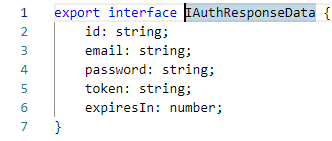
\includegraphics
	{../LaTeX/Images/implementare_iauthresponsedata.PNG}
	\caption{Interfața ”IAuthResponseData”}
	\label{fig:63}
\end{figure}

După înregistrare sau autentificare, utilizatorul este redirecționat către componenta ”Intakes”. ”Intakes” reprezintă tabloul de bord al aplicației și afișează numărul de calorii pe care acesta și le-a setat ca obiectiv de atins la momentul înregistrării.
De asemenea, oferă posibilitatea de a urmări istoricul utilizării aplicației, pe zile, ordonate de le cea mai îndepărtată zi, la cea mai apropiată. Acest istoric reprezintă de fapt jurnalul aportului de calorii al utilizatorului.

\begin{figure}[!htb]
	\centering
	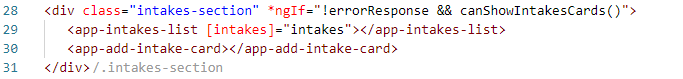
\includegraphics[width=0.9\textwidth]
	{../LaTeX/Images/implementare_intakes.PNG}
	\caption{Componenta ”Intakes”}
	\label{fig:64}
\end{figure}

Obiectul ”intakes” de la linia 29 din (Fig. \ref{fig:64}) este populat cu rezultatul unui request ”POST” către ”FoodSpyAPI” care întoarce o listă de intrări din jurnalul unui anume utilizator, identificat prin adresa acestuia de e-mail. 
Nu se face un request ”GET” deoarece acest endpoint din (Fig. \ref{fig:65}) permite sortarea intrărilor din jurnal, din punct de vedere cronologic, dacă se populează o proprietate numită ”sortOrder” cu valoarea 0 pentru ascendent sau cu valoarea 1 pentru descendent.

\begin{figure}[!htb]
	\centering
	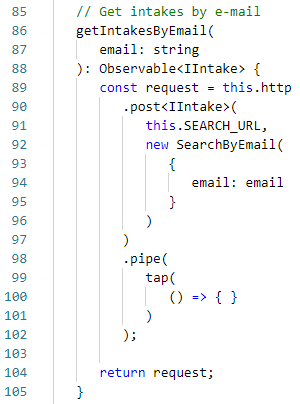
\includegraphics[width=0.6\textwidth]
	{../LaTeX/Images/implementare_getintakesbyemail.PNG}
	\caption{Request ”POST” către ”/api/db/intakes/search/”}
	\label{fig:65}
\end{figure}

În tabloul de bord, fiecare dintre aceste zile care face parte din istoric sunt conținute într-o componentă numită ”IntakeCard”. În ”IntakeCard”, istoricul nu este detaliat, afișează doar procentul de completare al aportului de calorii, și cantitatea totală de grăsimi, carbohidrați și zaharuri pe care utilizatorul le-a consumat în ziua respectivă.
\\ \\
Detaliile precum mâncărurile care fac parte din componența unei mese și cantitatea fiecăruia dintre mâncăruri consumate de utilizator sunt afișate în componenta ”IntakeHistory”, la care se ajunge prin intermediul unui hyperlink. Hyperlink-ul este atașat unei element ”<h2>” prin evenimentul ”(click)”, după cum se poate observa în (Fig. \ref{fig:66}). Elementul ”<h2>” exprimă numărul de mese consumate de utilizator într-o anumită zi.

\begin{figure}[!htb]
	\centering
	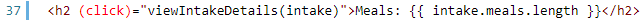
\includegraphics[width=0.95\textwidth]
	{../LaTeX/Images/implementare_hyperlink.PNG}
	\caption{Hyperlink atașat pe evenimentul ”(click)”}
	\label{fig:66}
\end{figure}

”Intakes” face legătură către ”AddMeal” prin componenta ”AddIntakeCard”. Cu ajutorul ”AddMeal”, un utilizator poate căuta mâncărurile pe care să la adauge la o masă, iar masa o poate adăuga la jurnalul din ziua respectivă.
\\ \\
”AddMeal” este cea mai complicată dintre componente, deoarece ea implementează funcționalitatea pentru căutarea mâncărurilor în baza de date și construcția unui obiect de tip ”IIntake”, care reprezintă o zi din jurnal.
\\ \\
Când utilizatorul accesează componenta ”AddMeal”, se inițializează obiectul de tip ”IIntake” cu valori default. De exemplu, o proprietate a acestui obiect este ”createdAt”, care va reține momentul la care s-a adăugat în jurnal prima masă. Se mai inițializează proprietatea ”email” cu e-mail-ul utilizatorului și ”targetCalories” cu obiectivul setat de utilizator.

\begin{figure}[!htb]
	\centering
	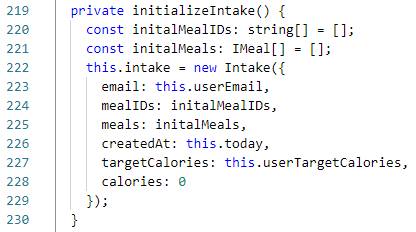
\includegraphics[width=0.8\textwidth]
	{../LaTeX/Images/implementare_initializeintake.PNG}
	\caption{Inițializarea componentei ”Intakes”}
	\label{fig:67}
\end{figure}

Căutarea mâncărurilor din baza de date se face folosind un ”<input>” de tip ”text” atașat la o funcție care preia termenul de căutare introdus de către utilizator și face un request ”GET” către ”FoodsService”. Termenul de căutare populează parametrul din URL numit ”name” și asta va determina endpoint-ul definit în ”FoodSpyAPI” să returneze o listă de mâncăruri filtrate după nume. Un exemplu de request ”GET” după criteriul numelui este ”/api/db/foods/search?name=ciocolata”.

\begin{figure}[!htb]
	\centering
	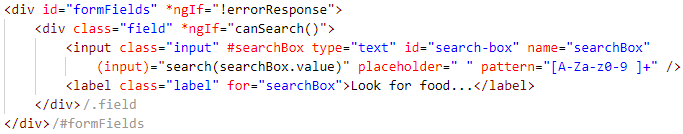
\includegraphics[width=0.9\textwidth]
	{../LaTeX/Images/implementare_search.PNG}
	\caption{Bara de căutare a mâncărurilor după nume}
	\label{fig:68}
\end{figure}

Odată găsită mâncarea în baza de date, utilizatorul poate deschide o căsuță de dialog, care reprezintă componenta ”EditFoodDialogue”. Aici, utilizatorul poate vedea mai multe detalii despre mâncarea selectată în urma căutării, printre care cantitatea de săruri sau proteine și de asemenea poate introduce cantitatea de mâncare, exprimată în grame.
\\ \\
Pentru cantitate este construită o validare care impune valoarea acesteia să nu poată depăși 1000 de grame. Validarea este ilustrată în (Fig. \ref{fig:69}). Aceasta poartă numele de ”foodQuantityValidator” și este implementată folosind clasa abstractă ”AbstractControl”. ”AbstractControl” permite accesul la valoarea introdusă de utilizator în formular și astfel se pot impune restricții asupra acesteia.

\begin{figure}[!htb]
	\centering
	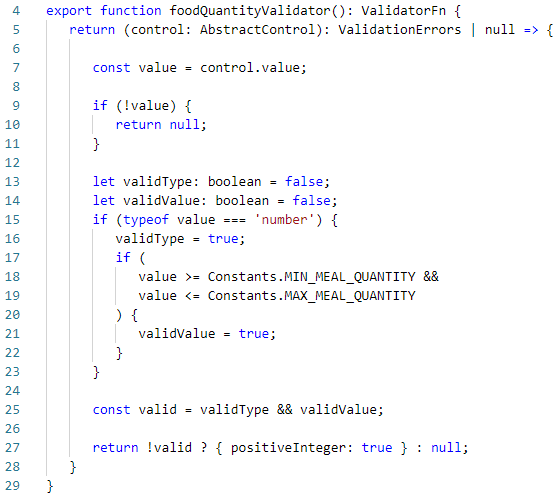
\includegraphics[width=0.9\textwidth]
	{../LaTeX/Images/implementare_foodqtyvalidator.PNG}
	\caption{Validarea pentru cantitatea de mâncare}
	\label{fig:69}
\end{figure}

După adăugarea unei mâncăruri, utilizatorul poate selecta tipul de masă pe care acesta a consumat-o. Tipurile de masă sunt ”Breakfast”, ”Lunch”, ”Dinner” sau ”Snack”. La momentul alegerii unuia dintre tipuri, formularul este valid și utilizatorului i se permite să înregistreze masa în jurnal.
\\ \\
Când se înregistrează o masă, există două scenarii.
\\ \\
Primul scenariu este acela în care utilizatorul nu are nicio intrare în jurnalul zilei respective, iar al doilea scenariu reprezintă modificarea unui jurnal deja existent.
În primul scenariu, implementarea este simplă deoarece este suficient să adăugăm masa în colecția ”Meals” din baza de date și apoi să introducem ID-ul acestei mese în proprietatea ”mealIDs” a obiectului de tip ”IIntake”. Ultimul pas este să trimitem un request ”POST” către ”FoodSpyAPI” pentru a înregistra jurnalul în colecția ”Intakes” din baza de date.
\\ \\
Al doilea scenariu este mai complicat deoarece în primul rând trebuie să determinăm dacă această masă nou adăugată face parte dintr-un tip de masă care există deja în obiectul ”IIntake”.
Dacă nu face parte, se persistă o masă nouă și se aduce referința în proprietatea ”mealIDs” prin ID, iar în final se execută un request ”PUT” pentru a modifica un ”Intake” deja existent. Dacă face parte, atunci trebuie identificată colecția de mese care are același tip cu tipul mesei pe care utilizatorul dorește să o adauge. După identificarea acesteia, se concatenează colecția existentă cu masa ce urmează să fie adăugată, se aduce referința (ID-ul) în obiectul ”IIntake” și din nou se modifică jurnalul (obiectul de tip ”IIntake”) prin același request ”PUT”.
\\ \\
După executarea oricăruia dintre cele 2 scenarii descrise mai sus, se reîncarcă pagina pentru a reflecta modificarea din obiectul ”IIntake”.

\begin{figure}[!htb]
	\centering
	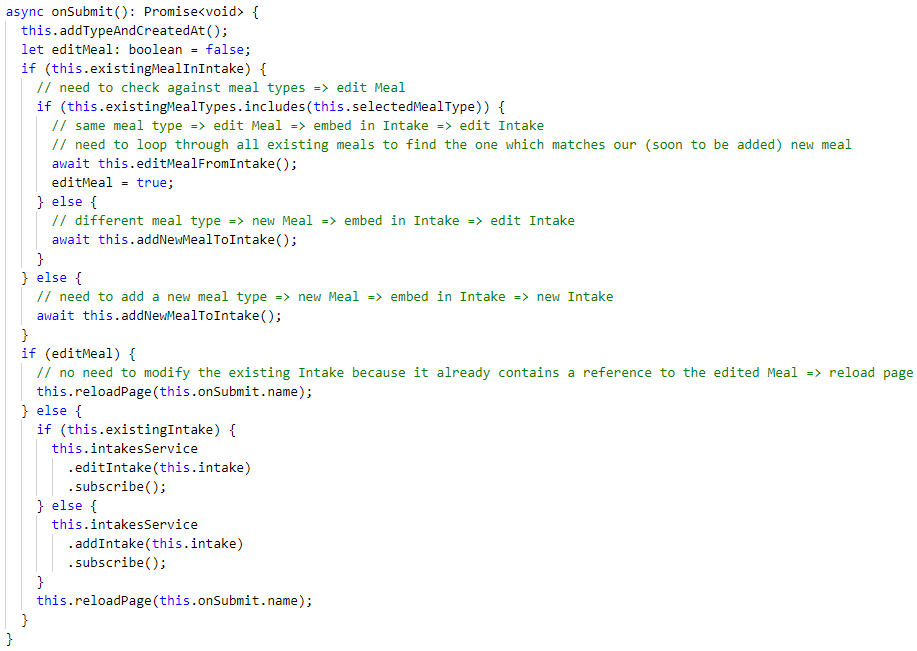
\includegraphics[width=0.95\textwidth]
	{../LaTeX/Images/implementare_addmeal.PNG}
	\caption{Adăugarea unei intrări în jurnalul zilnic}
	\label{fig:610}
\end{figure}

Prezent deasupra tuturor celorlalte componente, ”Header” (Fig. \ref{fig:611}) reprezintă antetul aplicației. Acesta afișează e-mail-ul utilizatorului autentificat, logo-ul aplicației și un buton pe care utilizatorul îl poate folosi pentru deconectare și redirecționare la componenta ”Auth”.

\begin{figure}[!htb]
	\centering
	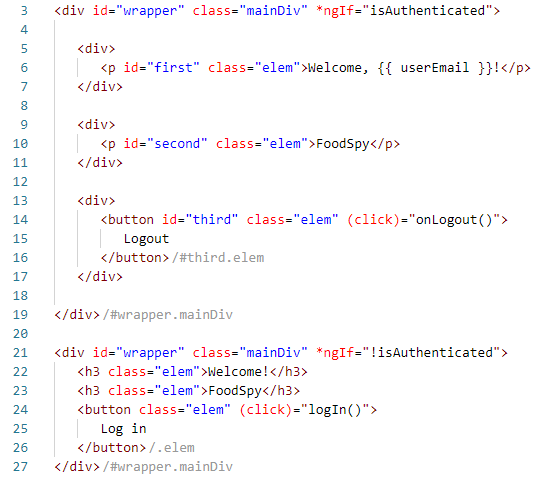
\includegraphics[width=0.8\textwidth]
	{../LaTeX/Images/implementare_header.PNG}
	\caption{Componenta ”Header”}
	\label{fig:611}
\end{figure}


\section{API pentru administrarea utilizatorilor}
Interfața de programare pentru administrarea utilizatorilor pune la dispoziție două endpoint-uri, un endpoint pentru operația de înregistrare a unui nou utilizator și unul pentru procesul de autentificare în aplicație.
\\ \\
La baza API-ului stă MikroORM, biblioteca TypeScript care implementează tehnica de a interoga și manipula datele dintr-o bază de date folosind o paradigmă orientată pe obiect. Cu ajutorul MikroORM, se definește o entitate care modelează profilul unui utilizator, dar și un manager peste această entitate care permite înregistrarea sau autentificarea acestuia în aplicație.
\\ \\
Pentru înregistrarea unui utilizator este nevoie să definim un endpoint pentru verbul ”POST” cu ajutorul unei rute. Din (Fig. \ref{fig:612}), se poate observa că ruta folosită pentru procesul de înregistrare este ruta rădăcină, adică ”/api/auth/register”.

\begin{figure}[!htb]
	\centering
	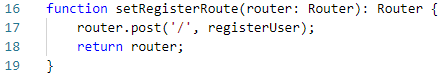
\includegraphics
	{../LaTeX/Images/userapi_rutaregister.PNG}
	\caption{Ruta pentru înregistrare}
	\label{fig:612}
\end{figure}

”registerUser” este funcția care face un apel către ”getUserByEmail” din ”UserService”. Funcția respectivă întoarce imediat o eroare dacă din corpul request-ului ”POST” lipsește e-mail-ul utilizatorului. Altfel, folosind manager-ul peste entități oferit de MikroORM, se caută utilizatorul identificat de e-mail-ul introdus în formularul din componenta ”Auth” din client. Dacă se găsește utilizatorul, detaliile despre acesta se returnează într-un obiect ”User”, iar dacă nu există, funcția întoarce ”null”.
\\ \\
În (Fig. \ref{fig:613}) este ilustrată funcția ”getUserByEmail”.

\begin{figure}[!htb]
	\centering
	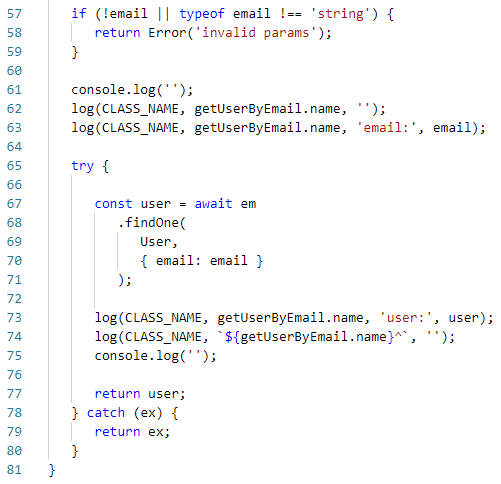
\includegraphics[width=0.9\textwidth]
	{../LaTeX/Images/userapi_getuserbyemail.PNG}
	\caption{Funcția ”getUserByEmail”}
	\label{fig:613}
\end{figure}

La momentul înregistrării, este important ca ”getUserByEmail” să returneze ”null”. Dacă returnează ”null”, înseamnă că utilizatorul nu există în baza de date și se poate înregistra cu succes folosind e-mail-ul, parola și obiectul caloric propus. Parola este criptată folosind biblioteca ”bcrypt” pentru a nu fi persistată în baza de date în format ”plain text”.
\\ \\
Dacă ”getUserByEmail” nu returnează ”null”, înseamnă că utilizatorului trebuie să îi fie afișat un mesaj de eroare care să-l atenționeze că există deja un cont creat cu același e-mail.

\begin{figure}[!htb]
	\centering
	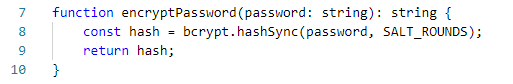
\includegraphics
	{../LaTeX/Images/userapi_bcrypt.PNG}
	\caption{Criptarea parolei folosind ”bcrypt”}
	\label{fig:614}
\end{figure}

Pentru autentificarea unui utilizator este nevoie să definim un endpoint pentru verbul ”POST” cu ajutorul unei rute. Din (Fig. \ref{fig:615}), se poate observa că ruta folosită pentru procesul de autentificare este ruta rădăcină, adică ”/api/auth/login”.

\begin{figure}[!htb]
	\centering
	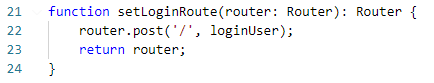
\includegraphics
	{../LaTeX/Images/userapi_rutalogin.PNG}
	\caption{Ruta pentru autentificare}
	\label{fig:615}
\end{figure}

Asemenea funcției ”registerUser”, funcția ”loginUser” face un apel către ”getUserByEmail” din ”UserService”.
\\ \\
La momentul autentificării, această funcție trebuie să returneze un obiect ”User”, care conține datele despre utilizator. În caz contrar, există scenariul în care utilizatorul nu există și trebuie mai întâi să se înregistreze sau există scenariul în care utilizatorul se află în baza de date. În acest caz, parola introdusă în formular este comparată cu parola persistată, iar dacă nu există o potrivire, un mesaj de eroare este afișat în client.

\begin{figure}[!htb]
	\centering
	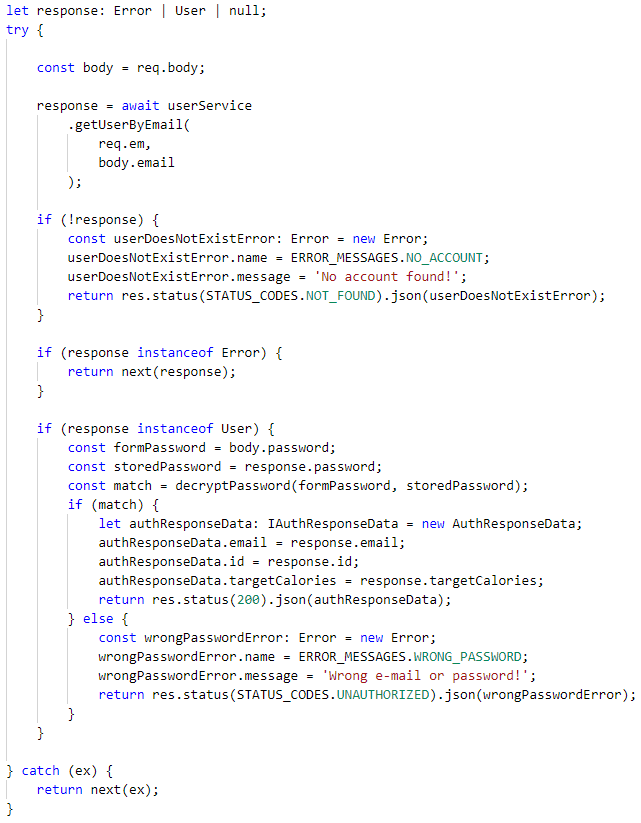
\includegraphics[width=0.9\textwidth]
	{../LaTeX/Images/userapi_loginuser.PNG}
	\caption{Corpul funcției ”loginUser”}
	\label{fig:616}
\end{figure}

La momentul pornirii server-ului care administrează datele despre utilizator, se caută un fișier numit ”.env” care conține string-ul de conectare la baza de date MongoDB precum și portul la care ascultă pentru cererile venite din partea clientului. ”.env” este interpretat de către API, care identifică string-ul de conectare și deschide portul de comunicare pentru client.
\\ \\
Fișierul ”.env” nu este înregistrat în repository-ul aplicației deoarece conține informații sensibile.


\section{API pentru gestiunea jurnalelor utilizatorilor}
Structura proiectului ”FoodSpyAPI” este reprezentată în (Fig. \ref{fig:616}).

\begin{figure}[!htb]
	\centering
	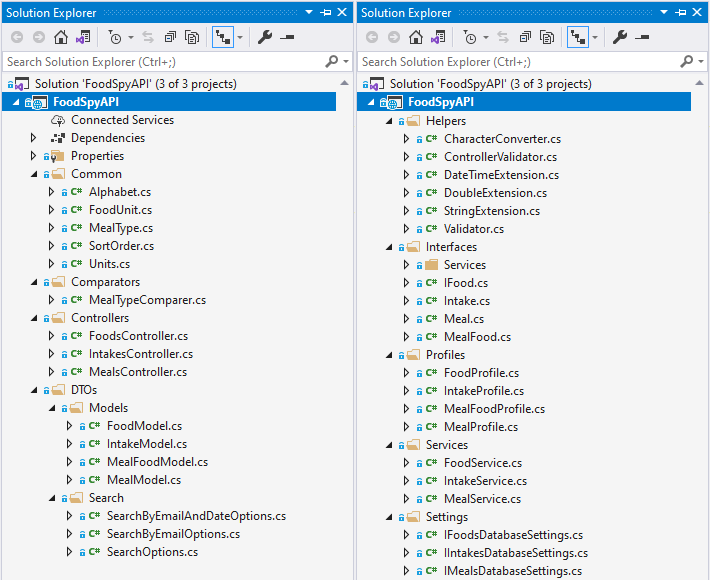
\includegraphics[width=0.8\textwidth]
	{../LaTeX/Images/fsapi_structura.PNG}
	\caption{Arhitectura proiectului ”FoodSpyAPI”}
	\label{fig:617}
\end{figure}

Directorul ”Common” conține clase și enumerări, precum ”Alphabet” sau ”MealType”. În ”Alphabet” există totalitatea caracterelor permise în aplicație, o reuniune a caracterelor alfabetului englez împreună cu literele cu diacritice din alfabetul limbii române. ”Alphabet” conține și o funcție ”ConvertDiacritic” care este utilizată pentru a îndepărta diacriticile dintr-un caracter.
\\ \\
”MealType” este o clasă statică care are în componența sa enumerarea ”MealType” folosită pentru definirea tipurilor de masă permise în aplicație. De asemenea, ”MealType” definește funcția ”GetMealTypesOrder” care are ca parametru de retur un ”Dictionary<string, uint>”. Dicționarul are ca utilitate sortarea meselor în funcție de tipul acestora, ”Breakfast” primul, ”Lunch” al doilea, ”Dinner” al treilea și ”Snack” ultimul.

\begin{figure}[!htb]
	\centering
	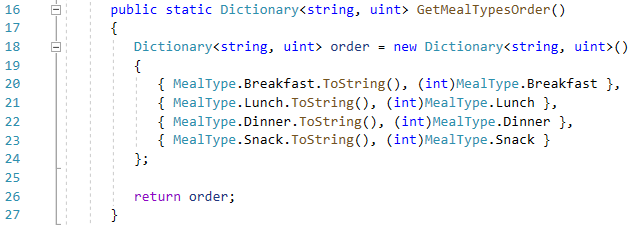
\includegraphics[width=0.8\textwidth]
	{../LaTeX/Images/fsapi_mealtype.PNG}
	\caption{Corpul funcției ”GetMealTypesOrder”}
	\label{fig:618}
\end{figure}

Dicționarul este folosit în funcția ”Compare” a clasei ”MealTypeComparer” din directorul ”Comparators”. În funcție de ponderea tipului de masă, clasa poate sorta mesele dintr-un jurnal în ordine crescătoare sau descrescătoare.

\begin{figure}[!htb]
	\centering
	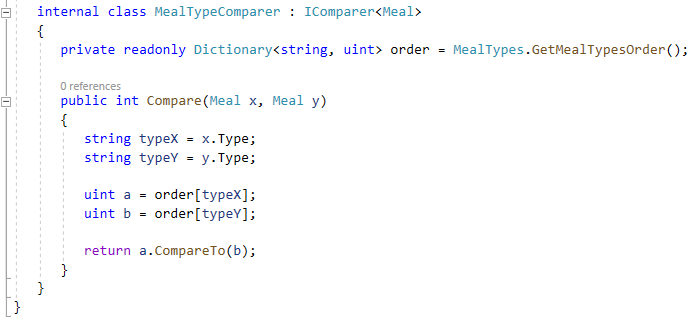
\includegraphics[width=0.8\textwidth]
	{../LaTeX/Images/fsapi_mealtypecomparer.PNG}
	\caption{Implementarea comparării tipurilor de mese}
	\label{fig:619}
\end{figure}

Interfața de programare pentru gestiunea jurnalelor utilizatorilor este compus din trei controller-e, ”IntakesController”, ”MealsController” și ”FoodsController”, din directorul ”Controllers”. Fiecare dintre acestea trei are definite endpoint-uri pentru verbele ”GET”, ”GET” cu parametrul din URL ”id”, ”POST”, ”PUT” și ”DELETE”.
\\ \\
”GET” returnează lista tuturor obiectelor de același tip cu tipul reprezentat de controller (”Intake”, ”Meal” sau ”Food”). ”GET” returnează un singur obiect identificat de parametrul ”id” din URL. ”POST” este folosit pentru adăugarea unui nou obiect, ”PUT” pentru editarea unui obiect deja existent, iar ”DELETE” pentru ștergerea unui obiect din baza de date.
\\ \\
Pentru implementarea anumitor endpoint-uri este nevoie mai mult de unul din aceste verbe. Spre exemplu, pentru ”PUT” trebuie mai întâi să inițiem un request ”GET” după parametrul ”id” din URL. Rezultatul acestui request va fi un obiect care ulterior poate fi modificat cu ajutorul request-ului ”PUT”.
\\ \\
Utilizatorul poate filtra mâncărurile din baza de date după criteriul numelui. De această filtrare se ocupă ”FoodsController” și funcția ”SearchFoodsByName”, ilustrată în (Fig. \ref{fig:620}). Această funcție primește ca parametru un obiect de tip ”string” care reprezintă termenul de căutare primit de la client. Cu ajutorul acestei funcții, a verbului ”GET” și a rutei ”/api/db/foods/search” se definește endpoint-ul care filtrează mâncărurile.

\begin{figure}[!htb]
	\centering
	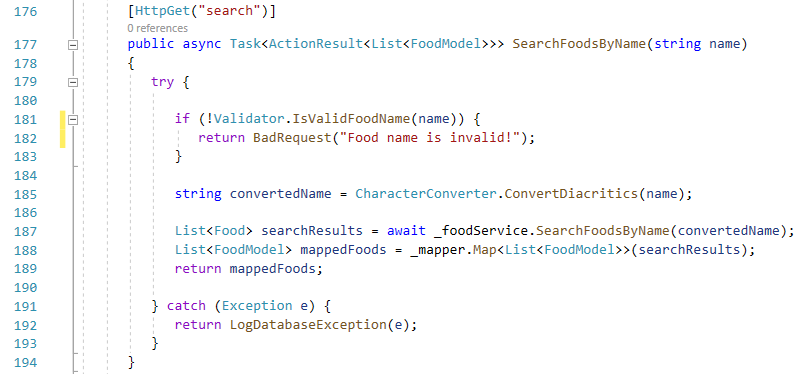
\includegraphics[width=0.9\textwidth]
	{../LaTeX/Images/fsapi_searchfoods.PNG}
	\caption{Corpul funcției ”SearchFoodsByName”}
	\label{fig:620}
\end{figure}

Se poate observa că prima oară se validează numele introdus de către utilizator și se returnează ca răspuns un ”status code” cu numărul 400, așa numitul ”BadRequest” și mesajul de eroare ”Food name is invalid!”, dacă numele nu este valid.
\\ \\
În următorul pas, se îndepărtează diacriticile și se apelează ”SearchFoodsByName” din ”FoodService”. Aici, se construiește un filtru care nu ține cont de stilul de scriere a numelui (”case insensitive”) și se interoghează baza de date. Rezultatul sau rezultatele căutării sunt returnate pentru a putea fi afișate utilizatorului și pentru a-i permite să adauge mâncarea la o masă din jurnal.
\\ \\
Dacă nu sunt rezultate în urma căutării, se returnează o listă goală pe care clientul o interpretează cu un mesaj de informare și anume ”No matching foods found”.

\begin{figure}[!htb]
	\centering
	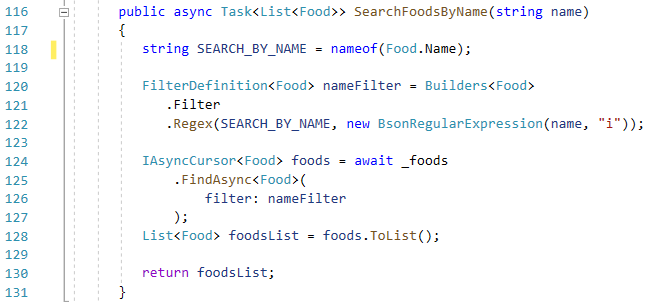
\includegraphics
	{../LaTeX/Images/fsapi_foodservice.PNG}
	\caption{Funcția ”SearchFoodsByName” din ”FoodService”}
	\label{fig:621}
\end{figure}

În directorul ”DTOs” sunt așa numitele ”data transfer objects”. Aceste obiecte sunt folosite strict pentru comunicarea între API și client. Acestea sunt o versiune simplificată a modelelor propriu-zise de date pentru a nu îngreuna transferul datelor cu proprietăți (informații) care nu sunt absolut necesare.
\\ \\
De exemplu, clasa care modelează o masă se numește ”Meal” și are definite proprietățile din (Fig. \ref{fig:622}). Din obiectul de transfer ”MealModel”, lipsește proprietatea ”List<Food> Foods”, după cum se poate observa din (Fig. \ref{fig:623}).

\begin{figure}[!htb]
	\centering
	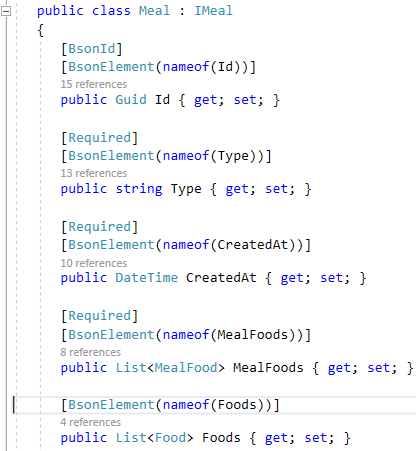
\includegraphics
	{../LaTeX/Images/fsapi_meal.PNG}
	\caption{Clasa ”Meal”}
	\label{fig:622}
\end{figure}

\begin{figure}[!htb]
	\centering
	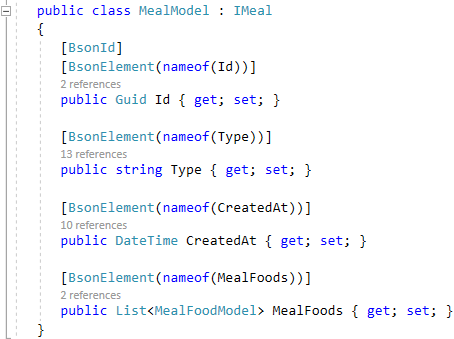
\includegraphics
	{../LaTeX/Images/fsapi_mealmodel.PNG}
	\caption{Clasa ”MealModel”}
	\label{fig:623}
\end{figure}

Tot în directorul ”DTOs” există clase care facilitează construirea unor request-uri ”POST” pentru filtrarea obiectelor de tip ”Intake”, spre exemplu după e-mail și după o anumită dată, cum este cazul clasei ”SearchByEmailAndDateOptions”.
\\ \\
Directorul ”Helpers” conține clase ajutătoare, precum ”CharacterConverter”, care poate lua un obiect de tip ”string” și îndepărta diacriticele din caracterele care compun respectivul string.
\\ \\
Cea mai des folosită clasă din acest director este ”Validator”, o clasă statică plină de funcții statice care sunt folosite pentru validare, printre care funcția care verifică validitatea unui ”id”, funcția care întoarce ”false” dacă e-mail-ul introdus de utilizator nu este sub o anumită formă, funcție care trece un string prin alfabetul descris în ”Alphabet” și verifică existența unor caractere nepermise și funcția care este folosită pentru a verifica faptul că un anumit tip de masă este prezent în enumerarea ”MealType”.

\begin{figure}[!htb]
	\centering
	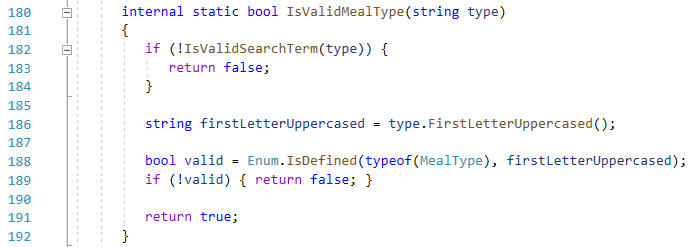
\includegraphics
	{../LaTeX/Images/fsapi_validmealtype.PNG}
	\caption{Funcția de validare a unui tip de masă}
	\label{fig:624}
\end{figure}

Tot în directorul ”Helpers” sunt metodele de extensie ”DateTimeExtension” și ”StringExtension”.
\\ \\
În ”StringExtension” este definită o metodă ”FirstLetterUppercased” care se aplică unui string și întoarce același obiect string, dar cu prima literă scrisă de tipar și restul cu literă mică. Această metodă este folosită spre exemplu la validarea unui tip de masă, după cum se poate observa în (Fig. \ref{fig:624}), la linia 186.
\\ \\
Corpul metodei ”FirstLetterUppercased” este ilustrat în (Fig. \ref{fig:625}).

\begin{figure}[!htb]
	\centering
	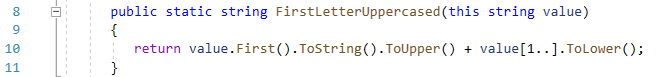
\includegraphics
	{../LaTeX/Images/fsapi_stringext.PNG}
	\caption{Metoda de extensie ”FirstLetterUppercased”}
	\label{fig:625}
\end{figure}

Interfețele care definesc setul minim de proprietăți pe care ar trebui să le aibă în componență modelele ”Food”, ”Meal” și ”Intake” se află în directorul ”Interfaces”. De exemplu, interfața ”IMeal” este reprezentată în (Fig. \ref{fig:626}).

\begin{figure}[!htb]
	\centering
	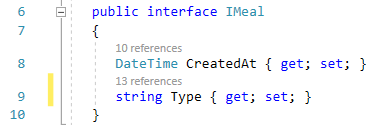
\includegraphics
	{../LaTeX/Images/fsapi_imeal.PNG}
	\caption{Interfața ”IMeal”}
	\label{fig:626}
\end{figure}

Clasele care se ocupă de asocierea proprietăților dintre modele și obiectele de transfer ale datelor se află în directorul ”Profiles”. ”MealProfile” este clasa care conține harta de asociere între ”Meal” și ”MealModel”. Această clasă este ilustrată în (Fig. \ref{fig:627}).

\begin{figure}[!htb]
	\centering
	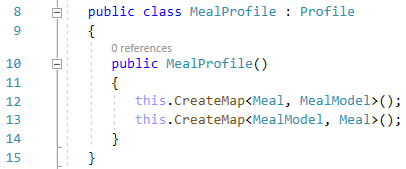
\includegraphics
	{../LaTeX/Images/fsapi_mealprofile.PNG}
	\caption{Clasa de asociere ”MealProfile”}
	\label{fig:627}
\end{figure}

Fiecare dintre controller-e are asociat un serviciu. Toate aceste servicii sunt reținute în directorul ”Services”. Serviciile sunt angajate de controller-e pentru a manipula datele din baza de date, în funcție de cererile care vin din partea clientului.
\\ \\
Serviciile mai sunt folosite și pentru a executa anumite operații auxiliare asupra datelor. Spre exemplu, în serviciul ”MealService” există funcția ”CalculateCalories” care preia ca parametru un obiect de tip ”Meal”, ia în calcul informațiile nutriționale ale mâncărurilor care se află în componența obiectului și calculează numărul de calorii consumate.
\\ \\
”CalculateCalories” este supraîncărcată de o versiune a funcției care primește ca parametru o listă de obiecte de tip ”Meal”. În (Fig. \ref{fig:628}) este reprezentată versiunea care primește un singur obiect ”Meal” ca parametru.

\begin{figure}[!htb]
	\centering
	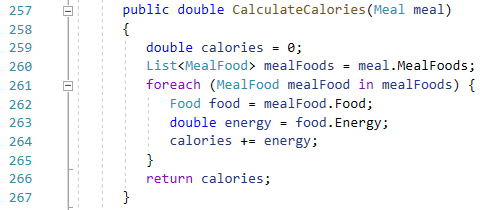
\includegraphics
	{../LaTeX/Images/fsapi_calccalories.PNG}
	\caption{Corpul funcției ”CalculateCalories”}
	\label{fig:628}
\end{figure}

Directorul ”Settings” conține interfețe și clase care facilitează accesul la colecțiile ”Foods”, ”Meals” și ”Intakes” din baza de date. Clasele conțin informații despre numele colecției, string-ul de conexiune și numele bazei de date, în acest caz ”FoodSpyDb”.


\section{Baza de date}
Baza de date a aplicației este ilustrată în (Fig. \ref{fig:629}).

\begin{figure}[!htb]
	\centering
	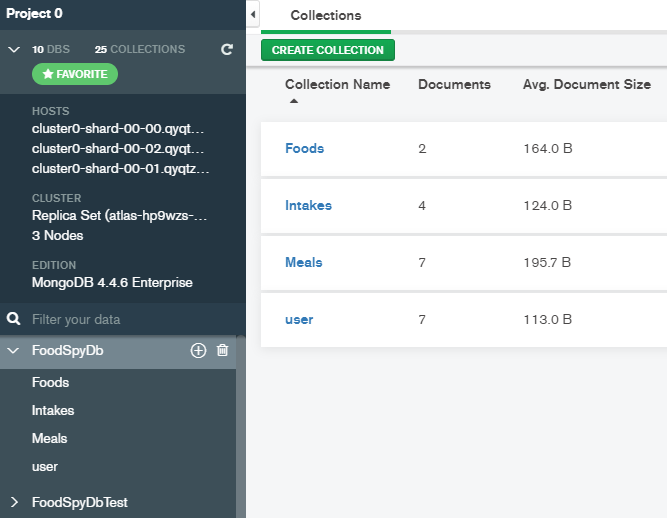
\includegraphics[width=0.9\textwidth]
	{../LaTeX/Images/db_collections.PNG}
	\caption{Colecțiile din baza de date}
	\label{fig:629}
\end{figure}

Baza de date conține 4 colecții de date. ”Foods” este colecția în care se rețin mâncărurile pe care utilizatorii le pot folosi pentru a le adăuga la o masă. Aceste mese sunt salvate în colecția ”Meals”. Mesele intră în componența unei zile din jurnal. O astfel de zi poartă numele de ”Intake” și este persistată în colecția ”Intakes”.
\\ \\
Există o relație între o entitate de tip ”Food” și o entitate de tip ”Meal” care nu este asociată cu niciun tabel în nivelul de persistență a datelor. Această relație poartă numele de ”MealFood” și are practic rolul unui tabel de legătură între ”Meal” și ”Food”. În relația ”MealFood” avem câmpurile ”mfid”, care reprezintă identificatorul unic al unei entități din ”Foods” și ”quantity” sau cantitatea acestui aliment exprimată în grame.
\\ \\
Cu ajutorul acestei relații, putem defini mai ușor mâncărurile care fac parte dintr-o masă. Dacă am fi salvat proprietatea de ”quantity” în entitatea ”Food”, nu am fi putut particulariza per masă în parte - toate mesele ar fi avut aceeași cantitate de mâncare definită în baza de date, iar utilizatorul nu ar fi putut introduce o cantitate diferită.
\\ \\
”user” este colecția în care sunt salvate datele despre utilizatori, respectiv e-mail-ul fiecăruia, parolele criptate folosind biblioteca ”bcrypt” și obiectivul caloric propus.